\TODO{Motivation}

\subsection{Random grid search algorithm}\label{sswwupgrade:opt_rgs}
The chosen algorithm for optimizing the event selection is known as the Random Grid Search (RGS) \cite{2018.rgs-paper}.
Consider a simple case of two variables $x$ and $y$ chosen to differentiate the signal from the background.
In order to be considered a signal event, a given event would be required to pass a \emph{cut point} $c = \{x > x_c, y > y_c\}$.
A simple method to choose the optimal cut point (i.e. the ``best'' values of the cuts $x_c$ and $y_c$) would be to construct an $n\times m$ rectangular grid in $x$ and $y$ consisting of points $(x_0,y_0), (x_1,y_1), ..., (x_n,y_m)$, as in Figure~\ref{fig:rgs_square_grid}.
One can then choose a cut point $c_k = \{x > x_i, y > y_j\}$ that maximizes the signal significance as measured by a chosen metric.
This would be considered a \emph{regular} or \emph{rectangular} grid search.

While effective in principle, this rectangular grid search comes with two major drawbacks:
\begin{enumerate}
\item The algorithm does not scale well as the number of variables to be optimized--the dimensionality of the grid--increases.  In the case of a square grid with $N$ bins per variable $v$, the number of cut points to be evaluated grows as $N^v$.
\item Signal and background samples are rarely evenly distributed over the entire grid, resulting in many cut points being sub-optimal and evaluating them would be a waste of computing resources.
\end{enumerate}

To combat these limitations, the RGS algorithm constructs a grid of cut points directly from the signal sample itself.
In the two-dimensional example, this means that the variables $x_i$ and $y_j$ making up the cut point $c_k = \{x > x_i, y > y_j\}$ take their values directly from a given signal event.
This has the benefit of creating a \emph{random grid} of cut points that is by construction  biased towards regions of high signal concentration.
This reduces the need for exponentially increasing numbers of cut points while ensuring that computing resources are not wasted in regions with few to no signal events.
An example of the the two-dimensional random grid is shown in Figure~\ref{fig:rgs_random_grid}.

\begin{figure}[htp]
  \centering
  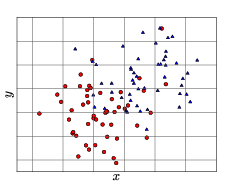
\includegraphics[width=0.48\textwidth]{figs/ssww_upgrade/rgs/figures_cuts_regulargrid}
  \caption{A visual representation of a rectangular grid search algorithm.  The signal events are the blue triangles, and the red circles are the background events. \TODO{replace with own figure}}   
  \label{fig:rgs_square_grid}
\end{figure}

\begin{figure}[htp]
  \centering
  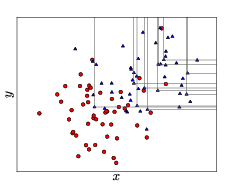
\includegraphics[width=0.48\textwidth]{figs/ssww_upgrade/rgs/figures_cuts_randomgrid}
  \caption{A visual representation of a random grid search algorithm.  The signal events are the blue triangles, and the red circles are the background events.  \TODO{replace with own figure}}   
  \label{fig:rgs_random_grid}
\end{figure}



\subsection{Inputs to the optimization}\label{sswwupgrade:opt_inputs}
Since the measurement of longitudinally polarized \ssww production is the focus of the upgrade study, the random grid was constructed using the LL-polarized events rather than the inclusive EWK production.
The variables chosen for optimization are:
\begin{itemize}
\item Leading lepton $\pt$
\item Dilepton invariant mass ($\mll$)
\item Leading jet $\pt$
\item Subleading jet $\pt$
\item Dijet invariant mass ($\mjj$)
\item Lepton-jet centrality ($\zeta$)
\end{itemize}

\subsection{Results of the optimization}\label{sswwupgrade:opt_results}
